\documentclass{beamer}

\usetheme{CambridgeUS}
\usecolortheme{orchid}

\usepackage[utf8]{inputenc}
\usepackage[T1]{fontenc}

% Math
\usepackage{amsmath}
\usepackage{amssymb}
\usepackage{bm}

% Graphics
\usepackage{graphicx}
\usepackage{caption}
\usepackage{subcaption}
\graphicspath{{../figs/}}

% Colors
\definecolor{darkblue}{HTML}{00688B}
\definecolor{darkgreen}{HTML}{6E8B3D}
\definecolor{cadet}{HTML}{DAE1FF}
\definecolor{salmon}{HTML}{FFB08A}

% Listings
\usepackage{textcomp}
\usepackage{listings}
\lstset{
  keywordstyle=\bfseries\color{orange},
  stringstyle=\color{darkblue!80},
  commentstyle=\color{darkblue!80},
  showstringspaces=false,
  basicstyle=\ttfamily,
  upquote=true,
}
\lstdefinestyle{fortran}{
  language=Fortran,
  morekeywords={for},
  deletekeywords={status},
}
\lstdefinestyle{c}{
  language=C,
  morekeywords={include},
}
\lstdefinestyle{shell}{
  language=bash,
}

\subtitle{TMA4280---Introduction to Supercomputing}

\begin{document}


\title{The tool: properties and flaws}
\author{Eivind Fonn}
\institute{SINTEF ICT / NTNU}
\date{December 2015}
\maketitle

\begin{frame}
  \frametitle{The tool}
  \begin{itemize}
    \item We here view the computer as a \emph{tool}---a means to reach a goal.
    \item Not a course in computer science, but a course in using this tool.
    \item No sane person would ever use the hammer without getting proper instructions!
  \end{itemize}
  \begin{center}
    \includegraphics[width=5cm]{wrong-tool-pizza} \\
    Image shamelessly stolen from the interwebs.
  \end{center}
\end{frame}

\begin{frame}
  \frametitle{Single processor systems: RISC architecture}
  \begin{center}
    \scalebox{0.8}{
      \begin{tikzpicture}[
  block/.style={
    draw=darkblue,
    fill=cadet,
    shape=rectangle,
    rounded corners=1mm,
    text height=1.5ex,
    text depth=.25ex,
  },
  l1/.style={
    minimum height=8mm,
    minimum width=4cm,
  },
  ops/.style={
    minimum height=8mm,
    minimum width=4cm,
    align=right,
  },
  inst/.style={
    minimum height=28mm,
    minimum width=16mm,
  },
  line/.style={
    thick,
    draw=darkblue,
  }]
  \node[block, l1] (L1inst) {L1 Instruction Cache};
  \node[block, l1, right=15mm of L1inst] (L1data) {L1 Data Cache};
  \node[block, l1, above=8mm of L1inst, fill=salmon] (Rest) {RAM, disk, network};
  \node[block, l1, above=8mm of L1data, fill=salmon] (L2) {L2 cache};
  \node[block, ops, below=16mm of L1data.east, anchor=east] (LS) {Load and store};
  \node[block, ops, below=10mm of LS.east, anchor=east] (Int) {Integer};
  \node[block, ops, below=10mm of Int.east, anchor=east] (Float) {Floating point};
  \node[block, inst, below=26mm of L1inst.east, anchor=east] (Decode) {Decode};
  \node[block, inst, below=26mm of L1inst.west, anchor=west] (Branch) {Branch};
  \node[block, inst, below=2mm of Decode, minimum height=8mm] (Clock) {Clock};

  \draw[line, <->] (Rest.east) -- (L2.west);
  \draw[line, <->] (L1inst.east) -- (L1data.west);
  \draw[line, <->] (L1data.south) -- (LS.north);
  \draw[line, ->] (Decode.east) -- (Int.west);
  \draw[line, ->] ([yshift=10mm]Decode.east) -- (LS.west);
  \draw[line, ->] ([yshift=-10mm]Decode.east) -- (Float.west);
  \draw[line, ->] (Decode.west) -- (Branch.east);
  \draw[line, ->] ([xshift=12mm]L1inst.south) -- (Decode.north);
  \draw[line, <-] ([xshift=-12mm]L1inst.south) -- (Branch.north);
  \draw[line] ($(L1inst.east)!0.5!(L1data.west)$) -- ($(Rest.east)!0.5!(L2.west)$);
\end{tikzpicture}

    }
  \end{center}
\end{frame}

\begin{frame}
  \frametitle{Single processor systems: memory hierarchy}
  \begin{center}
    \scalebox{0.8}{
      \begin{tikzpicture}[
  line/.style={
    thick,
    draw=darkblue,
  }]
  \coordinate (A) at (-4.5,0) {};
  \coordinate (B) at (4.5,0) {};
  \coordinate (C) at (0,7.4) {};
  \fill[cadet] (A) -- (B) -- (C);
  \draw[line, name path=AC] (A) -- (C);
  \draw[line, name path=BC] (B) -- (C);
  \foreach \y/\A in
  {0/Tape, 1/Distributed memory, 2/Local disk, 3/Main memory (RAM), 4/Cache, 5/Registers, 6/CPU}
  {
    \path[name path=horiz] (A|-0,\y) -- (B|-0,\y);
    \draw[line, name intersections={of=AC and horiz,by=P},
    name intersections={of=BC and horiz,by=Q}] (P) -- (Q)
    node[midway, above=1mm, text height=1.5ex, text depth=.25ex] {\A};
  }
\end{tikzpicture}

    }
  \end{center}
\end{frame}

\begin{frame}
  \frametitle{Single processor systems: memory hierarchy}

  Typical memory access times for the MIPS R14000 processor. The numbers
  represent number of clock cycles.
  \begin{center}
    \bgroup\def\arraystretch{1.2}
\begin{tabular}{rl}
  \hline
  Memory type & Clock cycles \\ \hhline{==}
  Registers & $1$ \\ \hline
  L1 cache & $2$--$3$ \\ \hline
  L2 cache & $10$--$12$ \\ \hline
  Main memory &  $100$--$200$ \\ \hline
  Message passing & $\mathcal{O}(10^3)$--$\mathcal{O}(10^4)$ \\ \hline
  Local disk & $\mathcal{O}(10^6)$ \\ \hline
\end{tabular}
\egroup

  \end{center}
\end{frame}

\begin{frame}
  \frametitle{Fixed point numbers}
  \begin{itemize}
  \item How to encode decimal numbers in the binary system?
  \item First alternative: Use $x$ bits to represent the stuff before the
    comma, and $y$ bits to represent the stuff after the comma, where $x+y = w$
    for a $w$ bit representation. This is called a fixed point representation.
  \item Problem: We get a fixed range of numbers we can represent; i.e.
    $2^x + 1 - 2^{-y}$ is the largest.
  \item Called fixed point since the point (the comma) is fixed. The
    \emph{absolute} accuracy is constant.
  \end{itemize}
\end{frame}

\begin{frame}
  \frametitle{Floating point numbers}
  \begin{itemize}
  \item A better idea is to let the comma position ``float''.
  \item Floating-point numbers have constant \emph{relative} accuracy.
  \item Allows us to represent a much larger range of numbers.
  \end{itemize}
  \begin{center}
    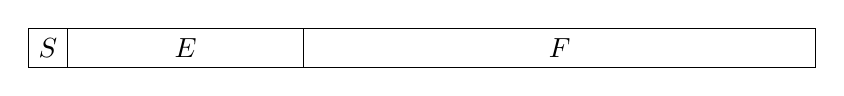
\begin{tikzpicture}[scale=0.5]
  \draw (0,0) rectangle (1,1);
  \draw (1,0) rectangle (7,1);
  \draw (7,0) rectangle (20,1);
  \node at (0.5, 0.5) {$S$};
  \node at (4, 0.5) {$E$};
  \node at (13.5, 0.5) {$F$};
\end{tikzpicture}

  \end{center}
  \begin{itemize}
    \item[S] The sign bit (1 bit).
    \item[E] The exponent
    \item[F] The mantissa
  \end{itemize}
\end{frame}

\begin{frame}
  \frametitle{Floating point numbers}
  Thus;
  \[
    V = (-1)^S \cdot 2^{E-B}\cdot M
  \]
  where the mantissa $M$ is defined as
  \[
    M = \underbrace{1}_{\times2^0} .
    \overbrace{\underbrace{b_1}_{\times2^{-1}}
      \underbrace{b_2}_{\times2^{-2}}\ldots}^{F}
  \]
  for normalized numbers (most common). Here $B$ is the \emph{bias}. Common
  precisions:
  \begin{center}
    \bgroup\def\arraystretch{1.2}
\begin{tabular}{ccccc} \hline
  Precision & $S$ & $E$ & $F$ & Total \\ \hhline{=====}
  Single & $1$ & $8$ & $23$ & 32
  \\ \hline
  Double & $1$ & $11$ & $52$ & 64
  \\ \hline
\end{tabular}
\egroup

  \end{center}
\end{frame}

\begin{frame}
  \frametitle{Floating point numbers}
  \begin{itemize}
  \item The \emph{bias} allows us to give a bias to large or small numbers
    (large or small exponents).
  \item Since we use a finite representation, we have a finite precision.
  \item Smallest and largest numbers:
    \begin{align*}
      V_\text{min} &= 1\cdot 2^{1-127}\cdot 1 = 2^{-126} = 1.17\ldots 10^{-38} \\
      V_\text{max} &= 1\cdot 2^{254-127}\cdot 2 = 3.40\ldots 10^{38}.
    \end{align*}
  \item More important: The smallest \emph{relative} difference between numbers
    we can represent
    \[
      2^{-23} = 1.19....10^{-7}.
    \]
    i.e.~under perfect circumstances we have about 7 digits of accuracy.
  \end{itemize}
\end{frame}

\begin{frame}
  \frametitle{Floating point operations}
  \begin{itemize}
    \item A very useful estimate for the size of a scientific code is the total
      number of floating point operations performed.
    \item Floating point operations: $+$, $-$, $\times$, $/$
    \item A floating point operation is called a Flop.
    \item It is tempting to use Flops for the plural, but that is \emph{not} the
      norm. Rather, Flops is used about Flop per second, which is a very useful
      performance metric.
    \item $\SI{3}{\flop}$ or $\SI{1}{\flop}$ (both Flop per second).
  \end{itemize}
\end{frame}

\begin{frame}
  \frametitle{Floating point limitations}
  \begin{itemize}
  \item We have a finite precision in our number representation. This leads to
    some issues.
  \item Subtraction: $1.2345\cdot 10^4$ minus $1.2344\cdot 10^4$.
    \begin{align*}
      & 1.2345 \cdot 10^4 - 1.2344 \cdot 10^4 \\
      &= (1.2345 - 1.2344) \cdot 10^4 \\
      &= \textcolor{red}{0.0001} \cdot 10^4 \\
      &= 1.0000 \cdot 10^0
    \end{align*}
    We have only a single digit of accuracy! This is called \emph{cancellation}.
  \item Example where this matters: Approximations of derivatives
    \[
      \frac{\text{d}f}{\text{d}x} \approx \frac{1}{h}\left( f(x+h) - f(x) \right)
    \]
  \end{itemize}
\end{frame}

\begin{frame}
  \frametitle{Floating point limitations}
  \begin{itemize}
  \item Additition: $1.2345\cdot 10^4$ plus $1.0000\cdot 10^0$.
    \begin{align*}
      & 1.2345 \cdot 10^4 + 1.0000 \cdot 10^0 \\
      &= (1.2345 + 0.0001) \cdot 10^4 \\
      &= 1.2346 \cdot 10^4
    \end{align*}
    OK!
  \item Additition: $1.2345\cdot 10^4$ plus $1.0000\cdot 10^{-1}$.
    \begin{align*}
      & 1.2345 \cdot 10^4 + 1.0000 \cdot 10^0 \\
      &= (1.2345 + 0.0000) \cdot 10^4 \\
      &= 1.2345 \cdot 10^4
    \end{align*}
    Adding the small number has no effect.
  \end{itemize}
\end{frame}

\begin{frame}[fragile]
  \frametitle{Pipelining vectorization}
  Consider the fused scalar multiplication and vector addition:
  \begin{align*}
    \bm c = \bm a + \gamma \bm b
  \end{align*}
  We can write this operation as the loop
  \begin{center}
    \begin{tabular}{c}
\begin{lstlisting}[style=fortran]
for i=1,n
  c(i) = a(i) + gamma * b(i)
end
\end{lstlisting}
    \end{tabular}
  \end{center}
  A single iteration is performed in a certain number of stages. These stages
  can be viewed as a pipeline.
\end{frame}

\begin{frame}
  \frametitle{Superscalar operations}
  \begin{align*}
    \bm c = \bm a + \gamma \bm b
  \end{align*}

  \begin{center}
    \begin{tikzpicture}[
  block/.style={
    draw=darkblue,
    fill=cadet,
    shape=rectangle,
    rounded corners=1mm,
    minimum height=12mm,
    minimum width=12mm,
  },
  pinin/.style={pin edge={to-, thick, darkblue}},
  pinout/.style={pin edge={-to, thick, darkblue}},
  ]
  \node[block, pin={[pinin]above:$\gamma$}, pin={[pinin]left:$b(i)$}] (mult) {$\times$};
  \node[block, right=20mm of mult, pin={[pinin]above:$a(i)$}, pin={[pinout]right:$c(i)$}] (add) {$+$};
  \draw[darkblue, ->, thick] (mult.east) -- (add.west);
\end{tikzpicture}
 \\
    Fused multiply and add (FMADD)
  \end{center}
\end{frame}

\begin{frame}
  \frametitle{Vectorization}
  Modern processors contain vector (SIMD, Single Instruction Multiple Data)
  units. This allows to apply the same operation to multiple data in parallel.
  In modern Intel (Sandy Bridge, Haswell) chips, the vector units are also
  superscalar (both AVX and SSE).

  Three ways to enable SIMD usage in your programs:
  \begin{itemize}
  \item autovectorizing compilers (ICC),
  \item hand-written assembly,
  \item intrinsics (built-in functions)
  \end{itemize}
\end{frame}

\begin{frame}
  \frametitle{Direct mapped cache}
  \begin{center}
    \input{\figs/direct-mapped-cache}
  \end{center}
  \[
    \text{Memory address} =
    \underbrace{b_1 \ldots b_k}_{\text{tag bits}}
    \underbrace{b_{k+1} \ldots b_{N}}_{\text{cache address}}.
  \]
\end{frame}

\begin{frame}[fragile]
  \frametitle{Direct mapped cache}
  \begin{center}
    \begin{tabular}{c}
\begin{lstlisting}[style=fortran]
for i=1,n
  c(i) = a(i) + b(i)
end
\end{lstlisting}
    \end{tabular}
  \end{center}

  If the vectors are precisely the same length as a cache line, we get cache
  trashing.

  \begin{center}
    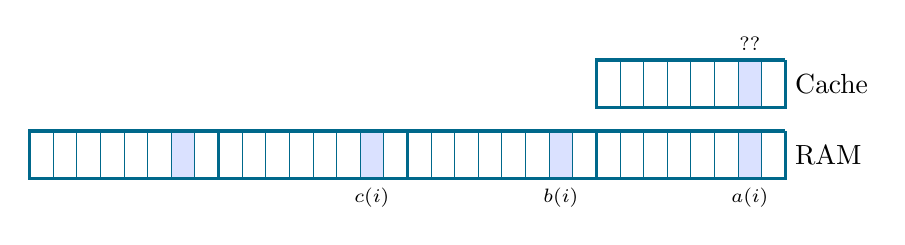
\begin{tikzpicture}[scale=0.3]
  \def \n {7};
  \def \k {3};
  \def \q {1};

  \foreach \i [
  evaluate=\i as \R using -(\n+1)*\i,
  evaluate=\i as \L using -(\n+1)*(\i+1),
  ] in {0,...,\k}
  {
    \fill[cadet] (\R-\q, 0) -- (\R-\q, -2) -- (\R-\q-1, -2) -- (\R-\q-1, 0) -- (\R-\q, 0);
    \draw[darkblue, very thick] (\R, 0) -- (\R, -2) -- (\L, -2) -- (\L, 0) -- (\R, 0);
    \foreach \j [
    evaluate=\j as \l using \R-\j
    ] in {1,...,\n}
    {
      \draw[darkblue, very thin] (\l, 0) -- (\l, -2);
    }
  }

  \fill[cadet] (-\q, 3) -- (-\q, 1) -- (-\q-1, 1) -- (-\q-1, 3) -- (-\q, 3);
  \draw[darkblue, very thick] (0, 3) -- (0, 1) -- (-\n-1, 1) -- (-\n-1, 3) -- (0, 3);
  \foreach \j in {1,...,\n} {
    \draw[darkblue, very thin] (0-\j, 3) -- (0-\j, 1);
  }

  \node[anchor=west] at (0, -1) {RAM};
  \node[anchor=west] at (0, 2) {Cache};
  \node[anchor=north] at (-\q-0.5, -2) {\scriptsize $a(i)$};
  \node[anchor=north] at (-\n-1-\q-0.5, -2) {\scriptsize $b(i)$};
  \node[anchor=north] at (-\n-\n-2-\q-0.5, -2) {\scriptsize $c(i)$};
  \node[anchor=south] at (-\q-0.5, 3) {\scriptsize ??};
\end{tikzpicture}

  \end{center}
\end{frame}

\begin{frame}
  \frametitle{Adjacent memory layout}
  \begin{center}
    
\begin{tikzpicture}[
  scale=0.8,
  every node/.style={
    text height=1.5ex,
    text depth=.25ex,
  }
  ]
  \draw[darkblue, very thick] (-6, 0) -- (6, 0);
  \draw[darkblue, very thick] (-6, 1) -- (6, 1);
  \draw[darkblue, very thin] (-3, 0) -- (-3, 1);
  \draw[darkblue, very thin] (-2, 0) -- (-2, 1);
  \draw[darkblue, very thin] (-1, 0) -- (-1, 1);
  \draw[darkblue, very thin] (0, 0) -- (0, 1);
  \draw[darkblue, very thin] (1, 0) -- (1, 1);
  \draw[darkblue, very thin] (2, 0) -- (2, 1);
  \draw[darkblue, very thin] (3, 0) -- (3, 1);
  \node at (-3.5, 0.5) {\footnotesize $\cdots$};
  \node at (-2.5, 0.5) {\footnotesize $a_i$};
  \node at (-1.5, 0.5) {\footnotesize $b_i$};
  \node at (-0.5, 0.5) {\footnotesize $c_i$};
  \node at (0.5, 0.5) {\footnotesize $a_{i+1}$};
  \node at (1.5, 0.5) {\footnotesize $b_{i+1}$};
  \node at (2.5, 0.5) {\footnotesize $c_{i+1}$};
  \node at (3.5, 0.5) {\footnotesize $\cdots$};
\end{tikzpicture}
 \\
    Interleaving the vectors in memory avoids cache trashing.
  \end{center}
\end{frame}

\begin{frame}
  \frametitle{Other cache strategies}
  \begin{itemize}
  \item Fully associative cache: \emph{all} bits in a memory address are used as
    tag bits, none of them as cache address. All cache addresses are available.
  \item $n$-way associative cache: uses $m$ fewer bits for cache address than a
    direct mapped cache, thus freeing up a choice of $n = 2^m$ cache addresses
    for each chunk. This is a good compromise between direct mapped cache and
    fully associative cache
  \end{itemize}
\end{frame}

\input{postamble}
